%========================
% Theme
%========================
\documentclass[8pt]{beamer}
\setbeamersize{text margin left=10mm,text margin right=10mm} 
\usetheme[progressbar=frametitle]{metropolis}
\usepackage{appendixnumberbeamer} % handles appendix slide numbering

%========================
% Packages: Icons and Tables
%========================
\usepackage{booktabs}        % professional tables
\usepackage[scale=1]{ccicons} % Creative Commons icons

%========================
% Packages: Plots and TikZ
%========================
\usepackage{pgfplots}
\usepgfplotslibrary{dateplot}

\usepackage{tikz}
\usetikzlibrary{positioning}

%========================
% Packages: Algorithms
%========================
\usepackage{algorithm}
\usepackage{algpseudocode}

%========================
% Packages: Math
%========================
\usepackage{amsmath,amsfonts,amsthm,amssymb}
\newtheorem{prop}{Proposition}

%========================
% Custom commands
%========================
\usepackage{xspace}
\newcommand{\themename}{\textbf{\textsc{metropolis}}\xspace}

%========================
% Custom footline
%========================
\setbeamertemplate{footline}
{%
  \leavevmode%
  \hbox{%
  \begin{beamercolorbox}[wd=.35\paperwidth,ht=2.5ex,dp=1.5ex,center]{author in head/foot}%
    \usebeamerfont{author in head/foot}\insertshortauthor
  \end{beamercolorbox}%
  \begin{beamercolorbox}[wd=.3\paperwidth,ht=2.5ex,dp=1ex,center]{title in head/foot}%
    \usebeamerfont{title in head/foot}\insertshorttitle
  \end{beamercolorbox}%
  \begin{beamercolorbox}[wd=.3\paperwidth,ht=2.5ex,dp=1ex,right]{date in head/foot}%
    \usebeamerfont{date in head/foot}\insertframenumber{} / \inserttotalframenumber
  \end{beamercolorbox}}%
  \vskip0pt%
}

%========================
% Remove default navigation symbols
%========================
\setbeamertemplate{navigation symbols}{}

\usepackage{pgf,pgfarrows,pgfnodes,pgfautomata,pgfheaps,pgfshade}
\usepackage{hyperref}
\usepackage{listings}
\usepackage{color}

\lstset{language=R,
    basicstyle=\small\ttfamily,
    stringstyle=\color{DarkGreen},
    otherkeywords={0,1,2,3,4,5,6,7,8,9},
    morekeywords={TRUE,FALSE},
    deletekeywords={data,frame,length,as,character},
    keywordstyle=\color{blue},
    commentstyle=\color{DarkGreen},
}

\usepackage{xcolor}

\lstset{
    language=Python,
    basicstyle=\ttfamily\small,
    keywordstyle=\color{blue},
    commentstyle=\color{gray},
    stringstyle=\color{red},
    breaklines=true,
    numbers=left,
    numberstyle=\tiny
}



%%%%%%%%%%%%%%%%%%%%%%%%%%%%%%%%%%%%%%%%%%%%%%%%%%%%%%%%%%%%%%%%%%%%
%%%%%%%%%%%%%%%%%%%%%%%%%%%%%%%%%%%%%%%%%%%%%%%%%%%%%%%%%%%%%%%%%%%%
% AQUI SE DEFINEN LAS IMAGENES PARA UTILIZAR DESPUES
%\pgfdeclareimage[interpolate=true, height=7cm,width=16cm]{halton-points}{halton-points}
%\pgfdeclareimage[interpolate=true, height=3cm, width =4cm]
%{serie-petroleo-reducido}{serie-petroleo-reducido}
%\pgfdeclareimage[interpolate=true, height=3cm, width =4cm]{rectangle-triangle}{rectangle-triangle}
%\pgfdeclareimage[interpolate=true, height=3cm, width =4cm]{any-angle}{any-angle}
%\pgfdeclareimage[interpolate=true, height=3cm, width =4cm]{Pythagoras}{Pythagoras}


\title{Chapter 1 - Random Number Generation}
\subtitle{Generation of Random Vectors, A geometric interpretation}
\author{Prof. Alex Alvarez, Ali Raisolsadat}
\institute{School of Mathematical and Computational Sciences \\ University of Prince Edward Island}
\date{} % leave empty or add \today
%\title[Stat 4110]{Stat 4110 Statistical Simulation}
%\subtitle{}
%\author[University of Prince Edward Island]{School of Mathematical and Computational Sciences \\ University of Prince Edward Island}

%========================
% Begin document
%========================
\begin{document}

%-------------------
% Title frame
%-------------------
\maketitle

%-------------------
% Slide 1:Connecting General Densities to Uniform Distributions
%-------------------
\begin{frame}{Connecting General Densities to Uniform Distributions}
The next result (Lemma 1.33 from the textbook) establishes a connection between distributions with general densities on $\mathbb{R}^d$ and uniform distributions on $\mathbb{R}^{d+1}$.

\vspace{2mm}

\textbf{Lemma}: Let $f: \mathbb{R}^d \rightarrow [0, \infty)$ be a probability density and let 
\begin{equation*}
A=\left\{(x,y) \in \mathbb{R}^d\times [0,\infty) : 0 \leq y <f(x)\right\} \subseteq \mathbb{R}^{d+1}
\end{equation*}

Then $|A|=1$ and the following two statements are equivalent:\\
\vspace{2mm}

a) $(X,Y)$ is uniformly distributed on $A$\\
\vspace{2mm}

b) $X$ is distributed with density $f$ on $\mathbb{R}^d$ and $Y=f(X)U$ where $U \sim U[0,1]$ independently of $X$.
\vspace{2mm}
\end{frame}

%-------------------
% Slide 2: Interpretation for One-Dimensional Densities
%-------------------
\begin{frame}{Interpretation for One-Dimensional Densities}
In the case $d=1$ we can easily interpret the previous result.

\vspace{2mm}

This Lemma could be used in both directions as needed:

\begin{itemize}
	\item \textbf{First implication}: Starting with a sample uniformly  distributed over $A$, we can look at the first component and get a sample that follows density $f$(this is very related to the usual sampling rejection algorithm).
Problem 2 from the homework uses this result.

\pause

	\item \textbf{Second implication}: We can sample from density $f$ and the uniform distribution to get a uniformly distributed sample over set $A$.
\end{itemize}

We could use the second implication in order to get uniformly  distributed samples over an \alert{unbounded} set $A$.
\end{frame}

%-------------------
% Slide 3: Example: Uniform Sampling Under a PDF Curve
%-------------------
\begin{frame}{Example: Uniform Sampling Under a PDF Curve}
\textbf{Example}: Generate a sample of 100 random points uniformly distributed under the curve of the probability density function of a standard normal random variable.

\vspace{2mm}

\alert{Algorithm}:

\begin{enumerate}
\item Generate $X \sim N(0,1)$
\item Compute $Z=pdf(X)$
\item Generate $Y \sim U[0, Z]$
\item Return $(X,Y)$
\end{enumerate}
\end{frame}

%-------------------
% Slide 4: Vectorized Implementation in R and Python
%-------------------
\begin{frame}[fragile]{Vectorized Implementation in R and Python}
\alert{Code}

\begin{columns}
\column{0.45\textwidth}
\textbf{R Code}

\begin{lstlisting}
n <- 1000;
X <- rnorm(n);
Z <- dnorm(X)
Y <- runif(n,min=0, max=Z)
plot(X,Y)
\end{lstlisting}

\column{0.50\textwidth}
\textbf{Python Code}

\begin{lstlisting}
import numpy as np
import matplotlib.pyplot as plt
from scipy.stats import norm

n = 1000
X = np.random.normal(size=n)
Z = norm.pdf(X)
Y = np.random.uniform(low=0, high=Z)

plt.scatter(X, Y)
plt.show()
\end{lstlisting}
\end{columns}

\vspace{2mm}

You can program this with a "for" loop instead, but it would be less efficient.
\end{frame}


%-------------------
% Slide 5: Visualizing the Uniform Sample Under a PDF
%-------------------
\begin{frame}{Visualizing the Uniform Sample Under a PDF}
Generated Sample uniformly distributed over the region under the density function of a standard normal random variable.

\begin{center}
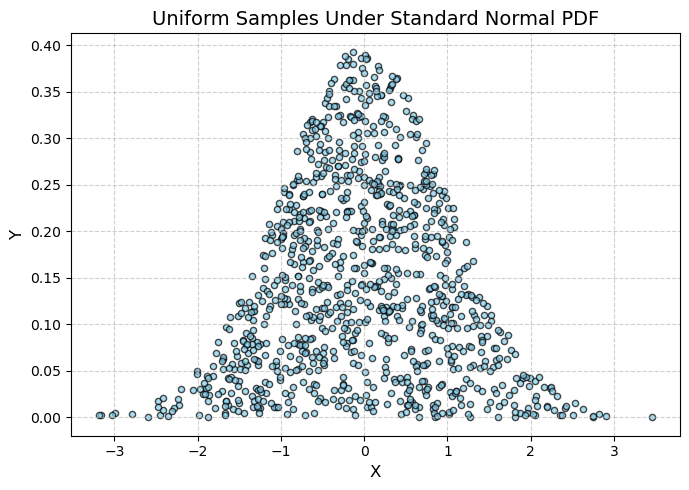
\includegraphics[scale=0.5]{chapter1-part5-plot1.png}
\end{center}
\end{frame}


%-------------------
% Slide 6: Remarks on the Uniform Sampling Method
%-------------------
\begin{frame}{Remarks on the Uniform Sampling Method}
\textbf{Remarks}:

\begin{itemize}
	\item This is a very straightforward method as long as we know how to sample from the density $f$.
	\item It can be applied also when $d \geq 1$, to both bounded and unbounded sets.
	\item By design the method only applies to sets $A$ with $|A|=1$ (meaning that area equals 1 for $d=1$, volume equals 1 for $d=2$, etc.) but we can modify it to also take into account other sets where $|A| \neq 1$.
\end{itemize}
\end{frame}

%-------------------
% Slide 7: Homework
%-------------------
\begin{frame}{Homework}
\begin{enumerate}
	\item Consider the probability density function given by $f(x)=\frac{1}{ (x+1)\ln 2}$ on $[0,1]$ and 0 otherwise. Define $B$ as follows
\begin{equation*}
B=\left\{(x,y) \in \mathbb{R}^2 : 0 \leq x \leq 1, 0 \leq y <f(x)\right\}
\end{equation*}
and let $A$ be the rectangle $A=\left\{(x,y) \in \mathbb{R}^2 : 0 \leq x \leq 1, 0 \leq y <1/\ln 2\right\}$

We can see that $B \subset A$.

a) Write a computer program that generates a random sample of 1000 uniformly distributed random points in $B$, by applying rejection sampling to uniformly distributed random points in $A$.

b) Use the outcome from part a) to get a random sample of 1000 random numbers with probability density $f$.
\end{enumerate}
\end{frame}

\end{document}